\documentclass{article}

\usepackage[margin=1.5in]{geometry}

\usepackage[urlcolor=blue]{hyperref}
\usepackage{listings}
\usepackage{tikz}
\usepackage{amsmath}
\usepackage{amssymb}
\usepackage{xcolor}

\DeclareMathOperator{\resNode}{res}
\DeclareMathOperator{\fracNode}{frac}
\DeclareMathOperator{\thresholdNode}{thres}
\DeclareMathOperator{\subscriptNode}{lookup}
\DeclareMathOperator{\readNode}{read}
\DeclareMathOperator{\dataNode}{data}
\DeclareMathOperator{\inputNode}{input}

\newcommand{\code}[1]{\texttt{#1}}
\newcommand{\todo}[1]{{\textcolor{red}{#1}}}

\begin{document}

\section{Motivation}

The current calculation system is long overdue for an overhaul.
It works well for baked-in sets of formulas but has shortcomings when specification involves more complicated procedures
For example, Ganyu's A1, which increases the Frost Flake CRIT Rate by 20\%, requires the Frost Flake calculation to use a new formula with a different CRIT Rate calculation instead of the preexisting one.
Using different formulas for similar calculations, such as in this scenario, also prevents the optimizer from merging those calculations.

The goal of the new formula engine includes

\begin{itemize}
	\item High flexibility when editing the formula, including when the operations may depend on one another,
	\item Ability to indicate that a portion of the code is reused at multiple places to avoid duplicate computations,
	\item Fast repeated calculations (comparable to the old one) where each round has slightly different parameters, and
	\item Ability to add multiple \emph{final formulas} together to form multi-variate optimization.
\end{itemize}

\section{Design}

The design of \emph{Waverider} takes a lot of inspirations from computational graph in TensorFlow\footnote{
	\url{https://www.tensorflow.org/guide/intro_to_graphs}
}.
It uses Directed Acyclic Graphs~(DAG) to represent formulas.
In particular, each node in the graph represents a single formula.
Some formulas rely on the values of another formulas, which we refer to as \emph{operands}.
This dependency is indicated using graph edges; edges leaving a node point toward its operands.

In this document, we omit the arrow heads for graph edges, and instead use the convention that the edges point downward, from higher nodes toward lower nodes.
Nodes with no outward edges are \emph{leaf nodes}, representing constants and variables.
Nodes with no inward edges are \emph{root nodes}.
They represent the final formulas that the entire graph represents.
Note that some graphs may have multiple root nodes.

Figure~\ref{fig:design:graph-example} shows an example of a computation graph, representing a formula~$3 + 8 * 7 * x$.
The leaf nodes are nodes~$3, 8, 7$, and~$x$, all representing either constants or variables.
The internal nodes are nodes~$+$ and~$*$.
The~$*$ node represents the product of its operands, i.e., the formula~$8 * 7 * x$, while the~$+$ node represents the sum~$3 + (8 * 7 * x)$, which is also the formula that the entire graph represents.
%
\begin{figure}
	\centering
	\begin{tikzpicture}
		\node {$+$}
		child { node {$3$} }
		child { node {$*$}
				child { node {$8$} }
				child { node {$7$} }
				child { node {$x$} }
			};
	\end{tikzpicture}
	\caption{Graph for $3 + 8 * 7 * x$}
	\label{fig:design:graph-example}
\end{figure}

We now discuss different types of available nodes in more details.

\section{Node Types}

We distinguish nodes into numerical nodes and string nodes, based on the type of values they return.
That is, numerical nodes represent formulas returning some numerical values, while formulas in string nodes return string values.
Numerical nodes are primary nodes in the computational graph as this structure is designed to perform numerical computation.
The string nodes are used primarily to maintain the states of the graph, such as the element type of the dmg, the type of the weapon that the character uses, etc.

Throughout this section, we use~$y$ for the value of the current node and~$x_1, x_2, \dots, x_n$ for the values of its operands.

\subsection{Constant Node}

Constant nodes are nodes that represent constant values of any kind, both numerical and string.
They have no children, and therefore are leaf nodes.
Nodes~$3, 8$, and~$7$ in Figure~\ref{fig:design:graph-example} are examples of constant nodes.

For numerical constant nodes, we use the constant values to represent those nodes.
For string nodes, we also use double quotes to distinguish them from variable names, e.g., ``sword", ``electro", and ``avg''.

\subsection{Compute Node}

Most of internal nodes are \emph{compute nodes}.
They are numerical nodes that compute their values using only the values of their numerical operands.
Supported formulas includes
%
\begin{itemize}
	\item Enemy Resistance~($\resNode$):
	      \begin{equation*}
		      y = \begin{cases}
			      1 - x_1/2,    & x_1 \in (-\infty, 0),  \\
			      1 - x_1,      & x_1 \in [0, 3/4),      \\
			      1/(1 + 4x_1), & x_1 \in [3/4, \infty),
		      \end{cases}
	      \end{equation*}
	\item Threshold~($\thresholdNode$):
	      \begin{equation*}
		      y = \begin{cases}
			      x_3, & x_1 \ge x_2,      \\
			      0,   & \text{otherwise},
		      \end{cases}
	      \end{equation*}
	\item Summation~($+$):~$y = \sum_i x_i$,
	\item Production~($*$):~$y = \prod_i x_i$,
	\item Maximum~($\max$):~$y = \max_i\{ x_i \}$,
	\item Minimum~($\min$):~$y = \min_i\{ x_i \}$, and
	\item Sum-Fractional~($\fracNode$):~$y = {x_1} / (x_1 + x_2)$.
\end{itemize}
%
Note that some formulas have a fixed number of operands, such as Enemy Resistance, while others support a variable number of operands, such as Summation.

\subsubsection{Subscript Node}

Subscript nodes are special compute nodes.
Each subscript node is accompanied by a dictionary.
It uses the only numerical operand~$x_1$ as an index to lookup the dictionary.
A subscript node with a dictionary~$X$ is denoted by~$\subscriptNode_X$.

\subsection{Read Nodes and Data Nodes}

For general graph modification, we use \emph{read nodes} and \emph{data nodes}.
Read nodes act as placeholders for portions of the graph that are not yet available during graph construction.
Data nodes then provide appropriate replacement for each read node during an operation called \emph{read operation}.
For more information on read operation, see Section~\ref{sec:operation:read}.

Each read node contains a string array \emph{key} used to identify nodes that it represents and an \emph{aggregation method} for combining all nodes that match the key into a single node.
The supported aggregation methods includes summation, production, minimum, and maximum.
Read nodes have no operands, and therefore are leaf nodes.
We denote each read node with key~$k$ and aggregation method~$a$ by~$\readNode_k^a$.

For some read nodes, the keys are combinations of an array string \emph{prefix} followed by a string computed using a string node called \emph{suffix}.
We denote such read nodes with prefix~$p$, suffix node~$s$, and an aggregated method~$a$ by~$\readNode_{p+s}^a$.
Note that the string node~$s$ in this case is not treated as an operand, and the read node~$\readNode_{p+s}^a$ remains a leaf node of the graph.


Data nodes specify the mapping that read nodes use to map their keys to appropriate nodes.
Each data node contains one or more \emph{data objects}, each of which is a dictionary mapping each key into a single node.
The data node has one operand, which is simply forwarded when evaluating, i.e.,~$y = x_1$.
We denote the data node with data objects~$X_1, X_2, \dots, X_n$ as~$\dataNode_{X_1, X_2,\dots, X_n}$.

\subsection{Priority Nodes}

Priority nodes are string nodes that uses the value of the first (string) operands that returns a non-empty string.
That is,

\begin{itemize}
	\item If~$x_1 \neq \emptyset, y = x_1$,
	\item If~$x_1 = \emptyset, x_2\neq\emptyset, y = x_2$,
	\item If~$x_1 = x_2 = \emptyset, x_3\neq\emptyset, y = x_3$,
	\item etc.
\end{itemize}

\section{Operations on Graph}

There are multiple optimizations one can do to a graph to reduce computation time and precompute portions of the graph.
This section list a few operations available on a graph.
Note that the graph is designed to be immutable (to avoid \emph{spooky action at a distance}\footnote{
	\url{https://en.wikipedia.org/wiki/Action_at_a_distance_(computer_programming)}
}), so most of the \emph{modifications} actually create a new graph that represents the modified formulas.

\subsection{Read Operation}
\label{sec:operation:read}

Read operations update the read nodes by replacing them with the (aggregated) nodes given by data nodes.
The operation is as followed,
\begin{enumerate}
	\item\label{enum:operation:read:step:iterate} For each read node~$\readNode_k^a$,
	\begin{enumerate}
		\item Finds all data nodes~$\{\dataNode_i\}_i$ among its ancestors,
		\item Map each data object~$D$ in each data node~$\dataNode_i$ using the key~$k$ to a node~$D[k]$, ignoring any data objects that do not contain the key~$k$,
		\item Check if there are at least one mapped nodes,
		      \begin{enumerate}
			      \item\label{enum:operation:read:step:replace} If there are mapped nodes, aggregate the mapped nodes using the aggregation method~$a$, and replace the read node with the aggregated method,
			      \item Otherwise, the read node remains unchanged, and the operation proceeds to the next read node,
		      \end{enumerate}
		\item If there are unconsidered read nodes, go back to Step~\ref{enum:operation:read:step:iterate},
	\end{enumerate}
	\item After all read nodes are considered, replace the data nodes with their operands.
\end{enumerate}
%
In Step~\ref{enum:operation:read:step:replace}, if the replaced node contains read nodes, they are also included in later iterations of Step~\ref{enum:operation:read:step:iterate}.

Figure~\ref{fig:modification:reading} illustrates the reading operation at a single read node.
In this setup, the operand of a data node~$\dataNode_{X,Y,Z}$ has one read node~$\readNode_k^+$.
Furthermore, we assume that~$X[k]$ and~$Z[k]$ exist, but~$Y[k]$ does not.
During the read operation, the read node looks up~$X[k], Y[k]$, and~$Z[k]$ and combines the matching nodes using its aggregation method,~$+$.
Since~$Y[k]$ does not exist, it is not included in the aggregated node.
%
\begin{figure}
	\centering
	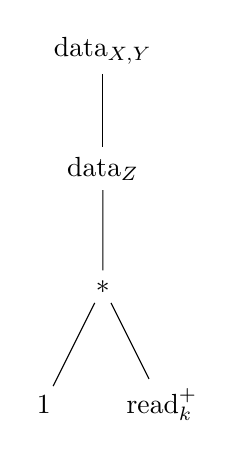
\begin{tikzpicture}[
			baseline=(current bounding box.east)
		]
		\node{$\dataNode_{X,Y}$}
		child { node {$\dataNode_{Z}$}
				child { node {$*$}
						child { node {$1$} }
						child { node {$\readNode_k^+$} }
					}
			};
	\end{tikzpicture}
	\quad$\Rightarrow$\quad
	\begin{tikzpicture}[
			baseline=(current bounding box.east)
		]
		\node{$*$}
		child { node {$1$} }
		child { node {$+$}
				child { node {$X[k]$} }
				child { node {$Z[k]$} }
			};
	\end{tikzpicture}
	\caption{Process of \emph{reading} $\readNode_k$ using~$\dataNode_{X, Y, Z}$ assuming~$X[k]$ and~$Z[k]$ exist and~$Y[k]$ does not}
	\label{fig:modification:reading}
\end{figure}

Note that during a read operation, all string nodes are evaluated and replaced with the appropriate values.
The rationale is that some read nodes require the values of the string node to be available as part of the key.

\subsection{Constant Folding}

The values of some nodes don't change across computations.
We can directly replace it with fewer computations, such as
%
\begin{itemize}
	\item If all operands of a node are Constant Nodes, we can replace it with the result of the calculation (as another Constant Nodes),
	\item We can apply read operation to each read node, and
	\item We can replace each data node with its only operand~($x_1$), after reading all read nodes.
\end{itemize}
%
Figure~\ref{fig:optimization:folding-example} shows an example of constant folding.
Since the formula~$1 + 2 * 3 * 4 + 3$ uses only constants in its computation, it can be replace with the result~$22$.
%
\begin{figure}
	\centering
	\begin{tikzpicture}[
			baseline=(current bounding box.east)
		]
		\node {$+$}
		child { node {$1$} }
		child { node {$*$}
				child { node {$2$} }
				child { node {$3$} }
				child { node {$4$} }
			}
		child { node {$3$} };
	\end{tikzpicture}
	\quad$\Rightarrow$\quad
	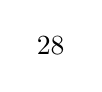
\begin{tikzpicture}[
			baseline=(current bounding box.east)
		]
		\node {$28$};
	\end{tikzpicture}
	\caption{Constant folding of~$1 + 2 * 3 * 4 + 3$  into~$28$}
	\label{fig:optimization:folding-example}
\end{figure}

\subsection{Flattening}

Some operations, such as summation and production, are commutative monoid\footnote{
	\url{https://en.wikipedia.org/wiki/Monoid\#Commutative_monoid}
}.
We can merge nodes with the same commutative monoid operation, e.g., as in Figure~\ref{fig:optimization:flatten-example}.
However, if an operand~$x_i$ is used by multiple nodes, we don't merge those operands; it is more efficient to keep such nodes separated.
%
\begin{figure}
	\centering
	\begin{tikzpicture}[
			baseline=(current bounding box.east)
		]
		\node {$*$}
		child[sibling distance = 80] { node {$*$}
				child[sibling distance = 40]  { node {$a$} }
				child[sibling distance = 40] { node {$b$} }
			}
		child[sibling distance = 80] { node {$*$}
				child[sibling distance = 40] { node {$c$} }
				child[sibling distance = 40] { node {$d$} }
			};
	\end{tikzpicture}
	\quad$\Rightarrow$\quad
	\begin{tikzpicture}[
			baseline=(current bounding box.east)
		]
		\node {$*$}
		child { node {$a$} }
		child { node {$b$} }
		child { node {$c$} }
		child { node {$d$} };
	\end{tikzpicture}
	\caption{Flattening of~$(a * b) * (c * d)$ into an equivalent~$a * b * c * d$}
	\label{fig:optimization:flatten-example}
\end{figure}

\subsection{Deduplication}

Some computations appear multiple times at different places in the hierarchy.
We can replace the duplicated nodes with either of the duplicates so they  share the result.
These nodes include
%
\begin{itemize}
	\item Read Nodes with the same key,
	\item Any nodes with the same dependencies in the same order, and
	\item Any commutative monoid nodes with the same dependencies in any order.
\end{itemize}
%
Furthermore, if any two commutative monoid nodes have more than one common dependency, we can separate common nodes into a nested operand.

Figure~\ref{fig:optimization:deduplicate} shows an example of deduplication on~$(1 + a + b) * \max(1 + a, c)$
In this figure, the the node~$1 + a + b$ and~$1 + a$ share the same part of the computation~$1 + a$.
The~$1 + a$ formula is then used to replace a portion of the formula~$1 + a + b$.
%
\begin{figure}
	\centering
	\begin{tikzpicture}[
			baseline=(current bounding box.east)
		]
		\node {$*$}
		child[sibling distance = 80] { node {$+$}
				child[sibling distance = 33] { node {$1$} }
				child[sibling distance = 33] { node {$a$} }
				child[sibling distance = 33] { node {$b$} }
			}
		child[sibling distance = 70] { node {$\max$}
				child[sibling distance = 30] { node {$+$}
						child { node {$1$} }
						child { node {$a$} }
					}
				child[sibling distance = 30] { node {$c$} }
			};
	\end{tikzpicture}
	\quad$\Rightarrow$\quad
	\begin{tikzpicture}[
			baseline=(current bounding box.east)
		]
		\node {$*$}
		child[sibling distance = 60] { node (parent) {$+$}
				child[sibling distance = 25] { node {$b$} }
				child[sibling distance=25, missing]
			}
		child[sibling distance = 70] { node {$\max$}
				child[sibling distance = 30] { node (child) {$+$}
						child { node {$1$} }
						child { node {$a$} }
					}
				child[sibling distance = 30] { node {$c$} }
			};
		\draw (parent) to[out=-70,in=130] (child);
	\end{tikzpicture}
	\caption{Deduplication of~$(1 + a)$ in~$(1 + a + b) * \max(1 + a, c)$}
	\label{fig:optimization:deduplicate}
\end{figure}

\section{Optimization}

After constructing the graphs, we can optimize the graph to reduce its size by performing the following operations in this particular order.
%
\begin{itemize}
	\item Perform a read operation on the graph,
	\item Perform all possible constant folding,
	\item Flatten all formulas, and
	\item Deduplicating all formulas that are used more than once.
\end{itemize}

\end{document}
